% !TEX TS-program = pdflatex
% !TEX encoding = UTF-8 Unicode

% This file is a template using the "beamer" package to create slides for a talk or presentation
% - Talk at a conference/colloquium.
% - Talk length is about 20min.
% - Style is ornate.

% MODIFIED by Jonathan Kew, 2008-07-06
% The header comments and encoding in this file were modified for inclusion with TeXworks.
% The content is otherwise unchanged from the original distributed with the beamer package.


\documentclass{beamer}

% No navigation symbols in bottom right corner
\beamertemplatenavigationsymbolsempty

\mode<presentation>
{
  \usetheme{Warsaw}
  % or ...

  \setbeamercovered{transparent}
  % or whatever (possibly just delete it)
}

\usepackage[english]{babel}
% or whatever

\usepackage[utf8]{inputenc}
% or whatever

\usepackage{times}
\usepackage[T1]{fontenc}
% Or whatever. Note that the encoding and the font should match. If T1
% does not look nice, try deleting the line with the fontenc.


\title[ID2205 Status Report] % (optional, use only with long paper titles)
{A Development Environment for DMDL, Status Report}

\author{Leon Fernandez}

\date{KTH Kista, Dec 2018}
% - Either use conference name or its abbreviation.
% - Not really informative to the audience, more for people (including
%   yourself) who are reading the slides online

\subject{}
% This is only inserted into the PDF information catalog. Can be left
% out. 



% If you have a file called "university-logo-filename.xxx", where xxx
% is a graphic format that can be processed by latex or pdflatex,
% resp., then you can add a logo as follows:

% \pgfdeclareimage[height=0.5cm]{university-logo}{university-logo-filename}
% \logo{\pgfuseimage{university-logo}}



\begin{document}

\begin{frame}
 	\titlepage
\end{frame}

\begin{frame}{Outline}
 	\tableofcontents
\end{frame}

\section{Intro}

\subsection{Background}

\begin{frame}{Software Defined Radios}
	What is it?
	\begin{itemize}
		\item<2-> Wideband transciever
		\item<3-> A ''reprogrammable'' radio
		\item<4-> Largely a KTH effort [SOURCES]
	\end{itemize}
\end{frame}

\begin{frame}{Software Defined Radios}
	Why SDRs?	
	\begin{itemize}
		\item<2-> Highly flexible
		\item<3-> Fast prototyping and implementation of protocols
		\item<4-> Wideband operation
	\end{itemize}
\end{frame}


\subsection{DMDL}
\begin{frame}{Brief Description}
	DMDL
	\begin{itemize}
		\item<2-> A graphical programming language
		\item<3-> Visually represent MAC layer protocols
		\item<4-> Synchronous Data Flow MoC
	\end{itemize}

	\onslide<5->{
	Read more
	\begin{itemize}
		\item SOURCE 1
		\item SOURCE 2
	\end{itemize}
	}
\end{frame}

\subsection{Motivation}

\begin{frame}{Why DMDL?}
	Most SDR flexibility exists only within the \textbf{PHY} layer.\\
	DMDL aims to extend the flexibility to the \textbf{MAC} layer.
\end{frame}

\begin{frame}{Why a Web DE?}
	Flexibility is the name of the game. \\
	If you have a browser, you can build a MAC protocol.
\end{frame}

\subsection{Goals}

\begin{frame}{Goals}
	\begin{itemize}
		\item<2-> Learning Outcomes
		\begin{itemize}
			\item<3-> MAC protocol simulation
			\item<4-> Preparation for thesis
		\end{itemize}

		\item<5-> Deliverables
		\begin{itemize}
			\item<6-> Simple web-based DE
			\item<7-> Syntax check
			\item<8-> (Optional) Export to platform-independent format (.xml) 
		\end{itemize}
	\end{itemize}
\end{frame}

\begin{frame}{NOT covered}
	\begin{itemize}
		\item<2-> No backend
		\begin{itemize}
			\item<3-> DE consists of HTML-, CSS- and JS-files and that's it
		\end{itemize}
		\item<4-> No platform integration
		\begin{itemize}
			\item<5-> Exports intermediate representation (.xml) and nothing more
		\end{itemize}
	\end{itemize}
\end{frame}

\section{Method}

\subsection{Languages}
\begin{frame}{Languages}
	First time doing web development
	\begin{itemize}
		\item<2-> Native JavaScript (ECS 5)
		\item<3-> HTML 5
		\item<4-> CSS 3
	\end{itemize}
\end{frame}

\subsection{Tools}
\begin{frame}{Tools}
	Keepin' it simple
	\begin{itemize}
		\item<2-> Firefox 63
		\item<3-> Gedit 3
	\end{itemize}
\end{frame}

\subsection{UML Code Overview}
\begin{frame}{UML Code Overview}
\centering
	\begin{figure}
 		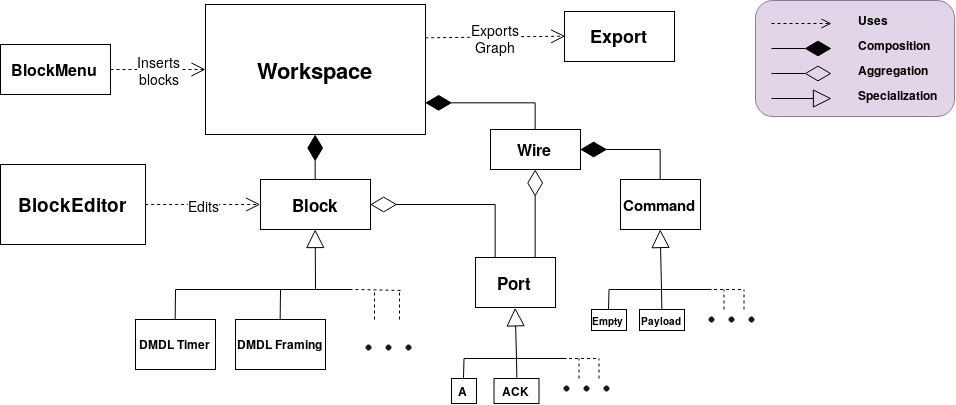
\includegraphics[width=\linewidth]{dmdl-editor.png}
		\caption{Overview of the code structure.}
		\label{fig:uml}
	\end{figure}
\end{frame}

\section{Status}

\subsection{Milestones}
\begin{frame}{Make Titles Informative.}
\centering
	\begin{tabular}{|c|c|c|} \hline
		\textbf{Milestone} & \textbf{Date} & \textbf{Status} \\ \hline
		Change appearance & Nov 2nd & Done \\ \hline
		Place blocks & Nov 7th & Done \\ \hline
		Block ports & Nov 12th & Done \\ \hline
		Connect ports & Nov 19th & Not Done \\ \hline
		Dropdown config & Nov 29th & Done \\ \hline
	\end{tabular}
\end{frame}


\subsection{UML Revisited}
\begin{frame}{Status in terms of UML}
\centering
	\begin{figure}
 		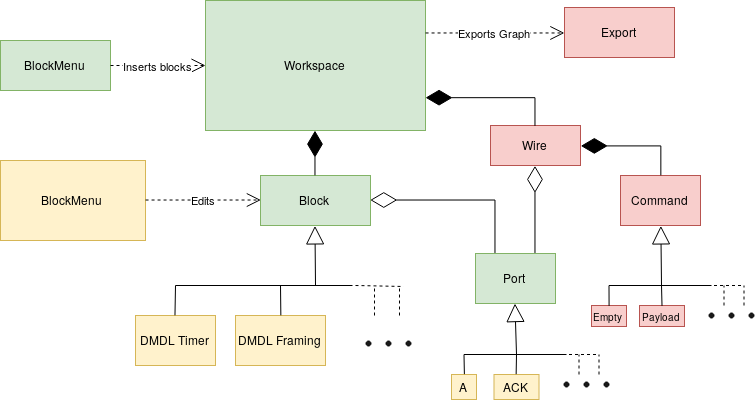
\includegraphics[width=\linewidth]{dmdl-editor-status.png}
 		\caption{Work status of the different classes.}
 		\label{fig:uml-status}
	\end{figure}
\end{frame}


\subsection{To Do}
\begin{frame}{Make Titles Informative.}
	What are the next steps?
	\begin{itemize}
		\item<2-> Wiring
		\item<3-> Block internals
	\end{itemize}
\end{frame}


\section*{Summary}
\begin{frame}{Summary}
\begin{itemize}
	\item Mostly on track, might have to do a bit of work during the holidays...
	\item DE right now is ''hollow''. No syntax check and no export.
	\item Git: \url{https://github.com/Zluudg/ID2205.git}
\end{itemize}
\end{frame}

\section*{Demo and Questions}
\begin{frame}{Demo and Questions}
\end{frame}


\end{document}


